
\documentclass[11pt,a4paper]{report}%especifica o tipo de documento que tenciona escrever: carta, artigo, relatório... neste caso é um relatório
% [11pt,a4paper] Define o tamanho principal das letras do documento. caso não especifique uma delas, é assumido 10pt
% a4paper -- Define o tamanho do papel.

\usepackage[portuges]{babel}%Babel -- irá activar automaticamente as regras apropriadas de hifenização para a língua todo o
                                   %-- o texto gerado é automaticamente traduzido para Português.
                                   %  Por exemplo, “chapter” irá passar a “capítulo”, “table of contents” a “conteúdo”.
                                   % portuges -- específica para o Português.
\usepackage[utf8]{inputenc} % define o encoding usado texto fonte (input)--usual "utf8" ou "latin1

\usepackage{graphicx} %permite incluir graficos, tabelas, figuras
\usepackage{url} % para utilizar o comando \url{}
\usepackage{enumerate} %permite escolher, nas listas enumeradas, se os iems sao marcados com letras ou numeros-romanos em vez de numeracao normal

%\usepackage{apalike} % gerar biliografia no estilo 'named' (apalike)

\usepackage{color} % Para escrever em cores
\usepackage{xcolor}

\usepackage{multirow} %tabelas com multilinhas
\usepackage{array} %formatação especial de tabelas em array

\usepackage[pdftex]{hyperref} % transformar as referências internas do seu documento em hiper-ligações.

% Para autómatos
\usepackage{tikz}
\usetikzlibrary{automata,arrows,positioning, arrows.meta, shapes.geometric}

\usepackage{amsmath,amssymb,amsfonts}
\usepackage{pdfpages}
\usepackage{float} % Image location specifier

%Exemplos de fontes -- nao e vulgar mudar o tipo de fonte
%\usepackage{tgbonum} % Fonte de letra: TEX Gyre Bonum
%\usepackage{lmodern} % Fonte de letra: Latin Modern Sans Serif
%\usepackage{helvet}  % Fonte de letra: Helvetica
%\usepackage{charter} % Fonte de letra:Charter

\definecolor{saddlebrown}{rgb}{0.55, 0.27, 0.07} % para definir uma nova cor, neste caso 'saddlebrown'

\usepackage{listings}  % para utilizar blocos de texto verbatim no estilo 'listings'
%paramerização mais vulgar dos blocos LISTING - GENERAL

%
%\lstset{ %
%	language=Java,							% choose the language of the code
%	basicstyle=\ttfamily\footnotesize,		% the size of the fonts that are used for the code
%	keywordstyle=\bfseries,					% set the keyword style
%	%numbers=left,							% where to put the line-numbers
%	numberstyle=\scriptsize,				% the size of the fonts that are used for the line-numbers
%	stepnumber=2,							% the step between two line-numbers. If it's 1 each line
%											% will be numbered
%	numbersep=5pt,							% how far the line-numbers are from the code
%	backgroundcolor=\color{white},			% choose the background color. You must add \usepackage{color}
%	showspaces=false,						% show spaces adding particular underscores
%	showstringspaces=false,					% underline spaces within strings
%	showtabs=false,							% show tabs within strings adding particular underscores
%	frame=none,								% adds a frame around the code
%	%abovecaptionskip=-.8em,
%	%belowcaptionskip=.7em,
%	tabsize=2,								% sets default tabsize to 2 spaces
%	captionpos=b,							% sets the caption-position to bottom
%	breaklines=true,						% sets automatic line breaking
%	breakatwhitespace=false,				% sets if automatic breaks should only happen at whitespace
%	title=\lstname,							% show the filename of files included with \lstinputlisting;
%											% also try caption instead of title
%	escapeinside={\%*}{*)},					% if you want to add a comment within your code
%	morekeywords={*,...}					% if you want to add more keywords to the set
%}

\usepackage{xspace} % deteta se a seguir a palavra tem uma palavra ou um sinal de pontuaçao se tiver uma palavra da espaço, se for um sinal de pontuaçao nao da espaço

\parindent=0pt %espaço a deixar para fazer a  indentação da primeira linha após um parágrafo
\parskip=2pt % espaço entre o parágrafo e o texto anterior

\setlength{\oddsidemargin}{-1cm} %espaço entre o texto e a margem
\setlength{\textwidth}{18cm} %Comprimento do texto na pagina
\setlength{\headsep}{-1cm} %espaço entre o texto e o cabeçalho
\setlength{\textheight}{23cm} %altura do texto na pagina

% comando '\def' usado para definir abreviatura (macros)
% o primeiro argumento é o nome do novo comando e o segundo entre chavetas é o texto original, ou sequência de controle, para que expande
\def\so{\emph{Sistemas Operativos}\xspace}
\def\titulo#1{\section{#1}}    %no corpo do documento usa-se na forma '\titulo{MEU TITULO}'
\def\area#1{{\em \'{A}rea: #1}\\[0.2cm]}
\def\resumo{\underline{Resumo}:\\ }

%\input{LPgeneralDefintions} %permite ler de um ficheiro de texto externo mais definições

\title{Sistemas Operativos\\
      2º Licenciatura em Ciências da Computação \\
      \textbf{Grupo 20 - Trabalho Prático}\\ SDStore: Relatório de Desenvolvimento
      } %Titulo do documento
%\title{Um Exemplo de Artigo em \LaTeX}
\author{Alef Keuffer\\ (A91683) \and Alexandre Baldé\\ (A70373)
         \and Ivo Lima\\ (A90214)
       } %autores do documento
\date{\today} %data

\begin{document} % corpo do documento
\maketitle % apresentar titulo, autor e data

\begin{abstract}  % resumo do documento
Neste relatório explicar-se-á a abordagem utilizada para construir o serviço de
armazenamento seguro de ficheiros SDStore, utilizando a linguagem C e os conhecimentos
práticos desenvolvidos nas UC de \so.
\end{abstract}

\tableofcontents % Insere a tabela de indice
\listoffigures % Insere a tabela de indice figuras
%\listoftables % Insere a tabela de indice tabelas

\chapter{Introdução} \label{chap:intro} %referência cruzada

Este relatório contém a descrição do projeto realizado pelo Grupo 20 para
o Trabalho Prático de Sistemas Operativos, para o ano letivo de 2021/2022.

\section*{Estrutura do Relatório}

A estrutura do relatório é a seguinte:
\begin{itemize}
\item No capítulo~\ref{chap:analysis} faz-se uma análise do comportamento dos
  programas cliente e servidor desenvolvidos para a aplicação SDStore.

\item No capítulo~\ref{chap:servidor} explicam-se alguns aspetos mais técnicos e concretos da implementação.

\item No capítulo~\ref{chap:bash_testes}, explica-se como compilar, executar e testar o projeto.

\item No capítulo~\ref{concl} termina-se o relatório com as conclusões e o trabalho futuro.
\end{itemize}

\chapter{Arquitetura da aplicação} \label{chap:analysis} %referência cruzada

\begin{figure}
  \centering
  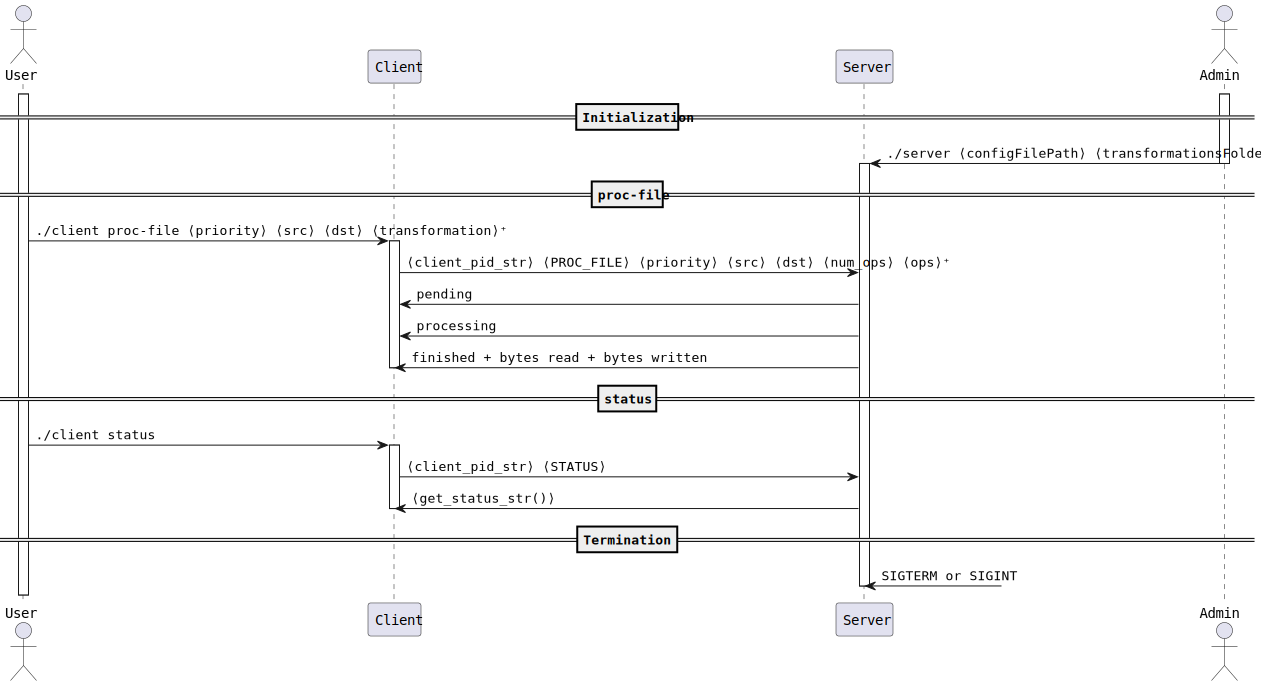
\includepdf[scale=0.66]{useExample1}
  \caption{Interação entre Cliente e Servidor via terminal}
\end{figure}

\newpage

\section{Notas sobre Cliente, Servidor}

\begin{itemize}
  \item A aplicação é composta por dois executáveis, \texttt{server} e \texttt{client}
  (que correspondem a \texttt{sdstore} e \texttt{sdstored}, resp.).
  \item Servidor:
  \begin{itemize}
    \item O servidor lê um ficheiro de configuração igual àquele descrito no enunciado,
    cuja informação ditará os limites de concorrência para cada transformação que pode correr.
    \item O servidor também precisa receber como argumento a pasta onde se encontram
    os programas que efetuam as transformações. Ou seja, como pedia o enunciado:
    \texttt{./server etc/sdstored.conf bin/sdstore-transformations}.
    \item A única forma de parar o servidor é enviar \texttt{SIGINT} ou \texttt{SIGTERM},
    o que não terminará quaisquer processos em curso, ou que já tenham sido submetidos por clientes.
  \end{itemize}

  \item Cliente:
  \begin{itemize}
    \item Tal como pedido no enunciado, o cliente pode submeter pedidos de transformação
    de ficheiros, com uma prioridade associada. A prioridade pode ser qualquer não negativo.
    \item O cliente também pode, através do comando \texttt{./client status}, ver quais são as
    transformações atualmente em curso, e quais os limites de concorrência do servidor.
  \end{itemize}
\end{itemize}

\section{Comunicação entre Servidor e Cliente}

\begin{itemize}
  \item Servidor e clientes comunicam entre si através de \texttt{mkfifo()}s.
  \item Existe um só FIFO para comunicação de todos os clientes para o servidor, chamado
  \texttt{SERVER}
  \item Cada cliente envia o seu PID em cada pedido que faz, porque:
  \item Cada cliente tem um FIFO próprio para receber informação relativa ao seu pedido, identificado
  pelo seu PID.

  \item \textbf{Cada cliente}, ao comunicar com o servidor, cria uma estrutura de dados~\ref{code:task_struct}
  com a informação relativa ao pedido (ou só \texttt{status} se for esse o caso), que depois envia ao servidor.\\
  O protocolo de comunicação entre cliente e servidor pode ser aproximado pela seguinte gramática:

\begin{align*}
  task\_message &::= \langle proc\_file \rangle\ |\ \langle status \rangle\ |\ \langle finished\_task \rangle \\
  \langle proc\_file \rangle &::= \langle client\_pid\_str \rangle \ \text{PROC\_FILE} \ \langle priority \rangle \langle src \rangle \langle dst \rangle \langle num\_ops \rangle \langle ops \rangle^+\\
  \langle status \rangle    &::= \langle client\_pid\_str \rangle \text{STATUS} \\
  \langle finished\_task \rangle &::= \text{FINISHED\_TASK} \langle monitor\_pid\_str \rangle \\
  \langle num\_ops \rangle &::= \langle int \rangle
\end{align*}
\label{text:protocol}

  \item O servidor não executa os pedidos que recebe dos clientes.\\
  Cria um \textbf{Monitor} por cada uma delas, que depois fica responsável por notificar o
  cliente e o servidor da sua terminação\label{text:monitor}. Ver imagem~\ref{fig:architecture}.

\end{itemize}


\newpage

\begin{figure}
\centering
\begin{tikzpicture}[shorten >=1pt,node distance=4cm,on grid, auto, initial text = ]

  \node[state, initial] (C2) {Client$_2$};
  \node[state, initial] (Cn) [right=of C2]{Client$_n$};
  \node[state, initial] (C1) [left=of C2]{Client$_1$};
  
  \node[state] (GlobFifo) [below=of C2]{Global FIFO};
  \node[state, initial] (Srv) [below=of GlobFifo]{Server};
  \node[state] (M2) [below=of Srv]{Monitor$_2$};
  \node[state] (M1) [left=of M2]{Monitor$_1$};
  \node[state] (Mn) [right=of M2]{Monitor$_n$};
  \node[rectangle,draw] (PQ) [right=of Srv]{PQueue};

  \path[->]
    (C1) edge node {$write(t_1)$} (GlobFifo)
    (C2) edge node {$write(t_2)$} (GlobFifo)
    (Cn) edge node {$write(t_n)$} (GlobFifo)
    (Srv) edge node {$read(t_k)$} (GlobFifo)
    (Srv) edge node[above] {$spawn(t_1)$} (M1)
          edge node {$spawn(t_2)$} (M2)
          edge node {$spawn(t_n)$} (Mn)
          edge [bend left] node {$pq\_insert(t_k)$} (PQ)

    (PQ) edge node {$t_j = pq\_pop()$} (Srv)

    (C2) -- node[auto=false]{\ldots} (Cn);

  \path
    (M2) -- node[auto=false]{\ldots} (Mn);


\end{tikzpicture}
\caption{Arquitetura global da aplicação}
\label{fig:architecture}
\end{figure}

Na figura \ref{fig:architecture}, vê-se uma especificação informal do funcionamento global
da aplicação.

\begin{itemize}
  \item Vários clientes podem comunicar em simultâneo com o servidor
  \item O servidor lê os pedidos do FIFO, insere-os na sua "\textit{priority queue}", e depois,
  de acordo com a sua lógica interna para controlar os limites de concorrência, cria monitores para as próximas
  tarefas, que ficam responsáveis pela "\textit{pipeline}" de transformações.
  \item São os monitores que comunicam ao cliente a conclusão da tarefa, como referido
  anteriormente~\ref{text:monitor}, assim como ao servidor, através de uma escrita no FIFO global de uma
  mensagem especial \texttt{FINISHED\_TASK}~\ref{text:protocol}.\\
  A figura seguinte ilustra melhor o funcionamento dos monitores.

\end{itemize}

\newpage

\begin{figure}
  \centering  
\begin{tikzpicture}[shorten >=1pt,node distance=4cm,on grid,auto, initial text = ]

  \node[state] (E12) {E$_{1,2}$};
  \node[state] (E11) [left=2cm of E12]{E$_{1,1}$};
  \node[state] (E1i) [right=2cm of E12]{E$_{1,i}$};

  \node[state, initial] (Mj)[below=of E12] {Monitor$_j$};

  \node[state] (GlobFifo) [below=of Mj]{Global FIFO};
  \node[state] (ClFifo) [right=6cm of Mj]{Client$_j$Fifo};
  \node[state] (Srv) [left=6cm of GlobFifo]{Server};
  \node[state] (Cj) [right=6cm of GlobFifo]{Client$_j$};

  \path[->]
    (Cj) edge node[pos=0.7] {$read("completed")$} (ClFifo)
    (Cj) edge node[right, pos=0.3] {$read("in = \ldots,\ out = \ldots")$} (ClFifo)
    (Srv) edge node {$read(done(t_j))$} (GlobFifo)
          edge [loop above] node {$update \ limits$} (Srv)
    (Mj) edge node[left] {$write(done(t_j))$} (GlobFifo)
         edge node {$pipe\_progs(t_j)$} (E11)
         edge node {$"completed"$} (ClFifo)
         edge node[below] {$"in = \ldots,\ out = \ldots"$} (ClFifo)
    (E11) edge node {} (E12)
    (E1i) edge node {execl()} (Mj);

    \path
    (E12) -- node[auto=false]{\ldots} (E1i);

\end{tikzpicture}
\caption{Relação entre Monitores, Clientes e Servidor}
\end{figure}

{\let\clearpage\relax \chapter{Funcionamento do servidor} \label{chap:servidor} } %capitulo e referencia cruzada

\begin{itemize}
  \item O servidor faz, essencialmente, um ciclo \lstinline{while(1) read(fifo);}.
  \item O servidor guarda os pedidos em execução numa lista, e utiliza "\lstinline{arrays}" para armazenar
  os limites de cada transformação, assim como o número de transformações em execução: ver anexo~\ref{code:server_struct}.
  \item Durante o desenvolvimento do projeto, consideraram-se alternativas que fariam os monitores enviar
  sinais ao servidor aquando do término da sua execução, para ser poder fazer \lstinline{waitpid(...)}, colher
  o processo monitor, e libertar os filtros em uso.\\
  \\
  No entanto, optou-se contra esta solução devido aos problemas de não-determinismo envolvidos no tratamento de sinais
  e.g. dois processos terminam exatamente ao mesmo tempo, só haverá um desses sinais na fila do servidor, só se fará
  \lstinline{wait} uma vez, etc.
  \item O servidor usa uma "\textit{priority queue}"\footnote{implementação disponível em \url{https://github.com/vy/libpqueue}}\label{footnote:pqueue}
  para guardar os pedidos que lê do FIFO global.
  \item Após cada monitor terminar e escrever no FIFO global que já o fez, o servidor lê essa mensagem do FIFO
  e atualiza depois os limites de concorrência de cada tipo de transformação.
  \item O servidor obtém a próxima tarefa a executar através de \lstinline{pqueue_peek()}. Se a próxima tarefa
  não puder ser executada, nunca se fazem esperas ativas: o servidor regressa à leitura do FIFO
  (que, recorde-se, é bloqueante), para esperar ou por novos pedidos de clientes, ou por monitores que terminam,
  levando à atualização dos limites de concorrência.
\end{itemize}

A imagem seguinte tem mais detalhes sobre a lógica interna do servidor.

\begin{figure}[H]
  \centering
  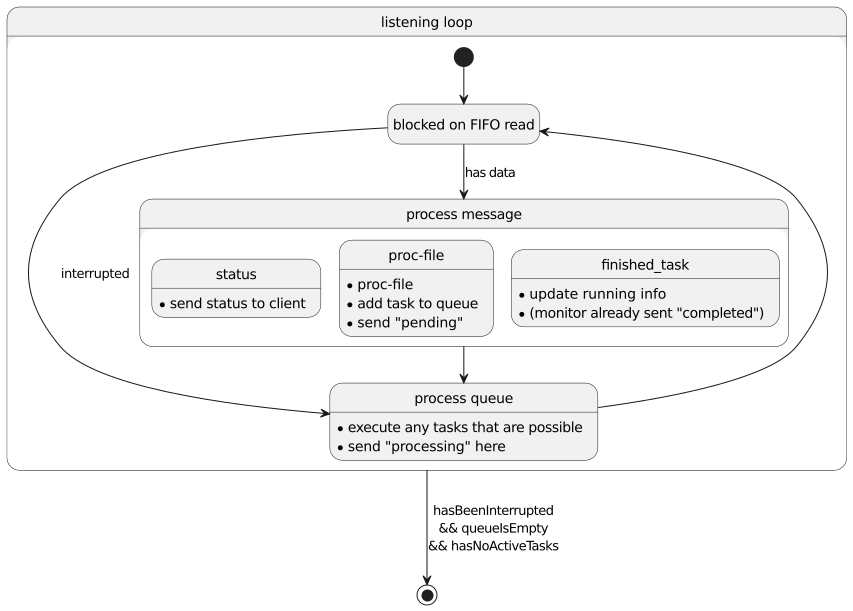
\includegraphics[scale=0.55]{loopLogic.png}
  \caption{Funcionamento interno do Servidor}
  \label{fig:server}
\end{figure}

Note-se que na figura acima~\ref{fig:server}, as mensagens que o servidor processa
correspondem ao protocolo definido em~\ref{text:protocol}:
\begin{itemize}
  \item \lstinline{status} para clientes que querem saber o estado do servidor
  \item \lstinline{proc-file} para submeter pedidos de processamento
  \item \lstinline{finished_task} para monitores que terminaram o pedido de um cliente.
\end{itemize}

\section{Funcionalidades Avançadas do Servidor}

Foram pedidas 3 funcionalidades avançadas para o serviço, que se enumeram de seguida.

\subsection{Tamanho de ficheiros de entrada/saída}
Para o servidor (através dos monitores que atribui a cada tarefa) reportar
o número de bytes lidos do ficheiro de \textit{input} e escritos no ficheiro de \textit{output},
faz-se somente \lstinline{lseek(fd, 0, SEEK_END)} para cada ficheiro.

\subsection{Terminação graciosa de servidor}
Para terminar de forma graciosa com \lstinline{SIGTERM/SIGQUIT}, executa-se, em cada processo monitor,
o código \lstinline{signal (SIGINT, SIG_IGN); signal (SIGTERM, SIG_IGN);}.\\
Caso contrário, \lstinline{CTRL^C} também os terminará \textemdash monitores são obtidos através de
\lstinline{fork()} do servidor, herdando o seu tratamento de sinais. \textemdash.\\
No servidor, faz-se

\lstset{language=C,
  basicstyle=\small, % print whole listing small
  keywordstyle=\color{pink}\bfseries\underbar,
  % underlined bold black keywords
  identifierstyle={\color{purple}},%
  commentstyle=\color{red}, % brown comments
  stringstyle=\color{blue}\ttfamily, % typewriter type for strings, blue 
  showstringspaces=true
}

\label{code:server_signal}
\begin{lstlisting}[caption={Tratamento de sinais no servidor}]
  void sig_handler (__attribute__((unused)) int signum) {
      unlink (SERVER);
      g.has_been_interrupted = 1;
  }

  struct sigaction sa;
  sigemptyset (&sa.sa_mask);
  sa.sa_handler = sig_handler;
  sa.sa_flags = 0;

  sigaction (SIGINT, &sa, NULL);
  sigaction (SIGTERM, &sa, NULL);
\end{lstlisting}

O comando \lstinline{unlink(SERVER)} previnirá mais clientes de fazer novos pedidos para o FIFO global.

\subsection{Prioridades de pedidos de processamento}

Como referido anteriormente, usa-se uma implementação de "\textit{priority queues}"~\ref{footnote:pqueue} em C
para decidir a ordem de execução dos pedidos.

Note-se que pedidos com a mesma prioridade não têm distinção, e o processo de escolha é não-determinístico.

\chapter{Testes realizados e Resultados} \label{chap:bash_testes} %capitulo e referencia cruzada

Para desenvolver e testar a aplicação, utilizaram-se as seguintes ferramentas:

\begin{itemize}
  \item Cmake: \url{https://cmake.org/}
  \item Tmux: \url{https://en.wikipedia.org/wiki/Tmux}
  \item Tmuxinator: \url{https://github.com/tmuxinator/tmuxinator}
  \item Git: \url{https://git-scm.com/}
\end{itemize}

O Tmuxinator utiliza configurações YAML (ver exemplos em anexo) que especificam cenários
de teste concretos, que depois podem ser executados através de scripts Bash que compilam
o projeto~\ref{code:compile_sh}, criam ficheiros de teste e depois executam os programas~\ref{code:test_sh}.\\

Para exemplificar, veja-se como obter, construir, e testar e.g. a concorrência do servidor (há outros cenários).
Assume-se que todas as ferramentas mencionadas estão instaladas e disponíveis no \texttt{PATH}.

\lstset{language=bash,
  basicstyle=\small, % print whole listing small
  keywordstyle=\color{pink}\bfseries\underbar,
  % underlined bold black keywords
  identifierstyle={\color{purple}},%
  commentstyle=\color{red}, % brown comments
  showstringspaces=true,
  % Without this it is not possible to have bash dollar signs inside \lstlisting.
  escapeinside=||
}
\begin{lstlisting}
git clone https://github.com/Alef-Keuffer/SDStore/
cd SDStore
chmod +x ./compile.sh
./compile.sh
cd tests
chmod +x ./test.sh
./test.sh conc
\end{lstlisting}

Para ver os testes disponíveis, ver~\ref{code:tmuxinator}.

\chapter{Conclusão} \label{concl}

Conclui-se desta forma a apresentação do Projeto Prático de \so do Grupo 20 para o
ano letivo 2021/2022.

\section{Comentários}

Terminar o projeto foi gratificante e transmitiu aos autores informação sobre como
arquitetar, estruturar e implementar pequenos programas em C que fazem uso de "\textit{system calls}".\\

No entanto, embora o Professor Paulo Almeida tenha dito, várias vezes e em tom humoroso, que o
trabalho se completaria numa tarde, os autores discordam.\\

Embora o projeto não chegue a ter 1000 LOC em C, e algumas centenas em \texttt{YAML/Bash},
foi completamente não-trivial projetar as aplicações servidor/cliente tendo em conta as restrições
impostas (comunicação através de FIFOs, pequeno conjunto de syscalls permissíveis, etc), e a novidade do
paradigma concorrente, que acrescenta os seus problemas \textemdash memória partilhada, sincronização,
limites de concorrência do servidor \textemdash e, cujas estratégias de abordagem não são abordados na parte
teórica da disciplina, e só parcialmente na parte prática.\\

Acresça-se a isto as dificuldades inerentes a "\textit{debugging}" em C, e todas as idiossincrasias da
linguagem, e este projeto foi facilmente o mais difícil que os autores completaram durante o curso inteiro.

\section{Trabalho Futuro}

Este projeto foi escrito num contexto académico, e não terá qualquer uso futuro adicional.

Se tivesse, a primeira necessidade seria melhor "\textit{error handling}".
Por exemplo, o servidor termina prematuramente se receber um pedido de uma transformação que
não exista.

\appendix % apendice
\chapter{Excertos de Código Utilizado no Projeto}

\lstset{language=C,
  basicstyle=\small, % print whole listing small
  keywordstyle=\color{pink}\bfseries\underbar,
  % underlined bold black keywords
  identifierstyle={\color{purple}},%
  commentstyle=\color{red}, % brown comments
  stringstyle=\color{blue}\ttfamily, % typewriter type for strings, blue 
  showstringspaces=true
}

\label{code:task_struct}
\begin{lstlisting}[language=bash, caption={Estrutura para pedidos de processamento de ficheiros}]
    typedef struct task_t {
      size_t pos; //private
      pqueue_pri_t pri;
      char *client_pid_str;
      char *src;
      char *dst;
      char *ops;
      int num_ops;
      pid_t monitor;
      char ops_totals[NUMBER_OF_TRANSFORMATIONS];
  } task_t;
\end{lstlisting}

\label{code:server_struct}
\begin{lstlisting}[caption={Amostra de Estrutura global do servidor}]
  struct {
    volatile sig_atomic_t has_been_interrupted;
    const int max_parallel_task;
    task_t *active_tasks[GLOBAL_MAX_PARALLEL_TASKS];
    const char *TRANSFORMATIONS_FOLDER;
    int server_fifo_rd;
    int server_fifo_wr;
    pqueue_t *queue;
    int num_active_tasks;
    int get_transformation_active_limit[NUMBER_OF_TRANSFORMATIONS];
    int get_transformation_active_count[NUMBER_OF_TRANSFORMATIONS];
  } g = {
      .has_been_interrupted = 0,
      .num_active_tasks = 0,
      .get_transformation_active_count = {0},
      .active_tasks = {NULL}
  };
\end{lstlisting}

\lstset{language=bash,%language=YAML, YAML is not supported!
  basicstyle=\small, % print whole listing small
  keywordstyle=\color{cyan}\bfseries\underbar,
  % underlined bold black keywords
  identifierstyle={\color{blue}},%
  commentstyle=\color{purple}, % brown comments
  showstringspaces=true,
  % Without this it is not possible to have bash dollar signs inside \lstlisting.
  escapeinside=||
}

\label{code:compile_sh}
\begin{lstlisting}[caption={Script Bash de compilação}]
  #!/bin/bash

  # Build SDStore executables, and return to project root.
  # Using subshell to avoid having to cd ..
  # https://www.shellcheck.net/wiki/SC2103
  (
      cd ./bin/sdstore-transformations || return;
      make clean;
      make;
  )
  
  # Build the project executables, and return to project's root.
  # Subshell, same as above.
  
  # If IDE cmake is working, this step may be skipped.
  mkdir -p build
  #cmake --build ./build --config Release --target all -j 18 --
  
  rm -f tests/server
  rm -f tests/client
  cp build/server tests
  cp build/client tests
  
  cp ./etc/sdstored.conf tests/sdstored.conf
  
  mkdir -p tests/bin
  cp -r ./bin/sdstore-transformations/* ./tests/bin/
  
\end{lstlisting}

\label{code:test_sh}
\begin{lstlisting}[caption={Script Bash de teste}]
  #!/bin/bash

  # How many test files to generate, both input and output.
  num_files=5
  
  # Size of each input file. Should be 10M+ to create scenarios with interesting delay.
  file_size="100M"
  
  for ((i=1;i<=num_files;i++)); do
      rm -f filein"|\$|i";
      rm -f fileout"|\$|i";
  done
  
  for ((i=1;i<=num_files;i++)); do
      head -c |\$|file_size </dev/urandom >filein"|\$|i";
      touch fileout"|\$|i";
  done
  
  # Argument passed to bash script dictates what test to run
  if [ "|\$|1" == "conc" ]; then
      tmuxinator start -p concurrency.yml
  elif [ "|\$|1" == "prio" ]; then
      tmuxinator start -p priority.yml;
  elif [ "|\$|1" == "status" ]; then
      tmuxinator start -p status.yml;
  elif [ "|\$|1" == "impossible" ]; then
      tmuxinator start -p impossible.yml;
  elif [ "|\$|1" == "ctrl_c" ]; then
      tmuxinator start -p ctrl_c.yml;
  else
    echo "Unknown test parameter! Please rerun with an appropriate argument."
  fi
\end{lstlisting}


\label{code:tmuxinator}
\begin{lstlisting}[caption={Exemplo de configurações Tmuxinator}]
  name: concurrency

  
  windows:
    - concurrency_and_limit:
        panes:
          - ./server sdstored.conf bin/
          - sleep 1; ./client proc-file 1 filein1 fileout1 bcompress bdecompress
          - sleep 1; ./client proc-file 1 filein2 fileout2 bcompress bdecompress
          - sleep 1; ./client proc-file 1 filein3 fileout3 bcompress bdecompress

  name: ctrl_c

  windows:
    - priority:
        panes:
          - ./server sdstored.conf bin/
          - sleep 1; ./client proc-file 1 filein1 fileout1 bcompress bcompress nop nop nop nop nop nop
          - sleep 1; ./client proc-file 3 filein2 fileout2 bcompress gcompress encrypt decrypt gdecompress bdecompress
          - sleep 2; ./client status; |\\| echo -e |\colorbox{blue!50}{CTRL\textasciicircum C IN SERVER}|;|\\| echo -e |\colorbox{pink!50}{``RUN ./client proc-file 1 filein1 fileout1 bcompress bcompress nop nop nop nop nop nop''}|

  name: priority

  # Resultado esperado: que o primeiro pedido bloqueie os outros, e que
  # o pedido com prioridade mais alta, feito no fim, corra em segundo lugar.
  windows:
    - priority:
        panes:
          - ./server sdstored.conf bin/
          - sleep 1; ./client proc-file 1 filein1 fileout1 nop nop nop nop nop nop bcompress
          - sleep 2; ./client proc-file 3 filein2 fileout2 nop bcompress gcompress gcompress
          - sleep 3; ./client proc-file 5 filein3 fileout3 nop bcompress gcompress gcompress

  name: impossible

  # Resultado esperado: que o servidor recuse o pedido por exceder os
  # limites de concorrencia para o comando gcompress.
  windows:
    - priority:
        panes:
          - ./server sdstored.conf bin/
          - sleep 2; ./client proc-file 1 filein1 fileout1 gcompress gcompress gcompress gcompress

  name: status

  # Resultado esperado: que o servidor mostre a segunte informacao.
  # [...] Message sent to 'SERVER'
  # Number of active tasks: 2
  # task [pid=...]: proc-file 1 filein1 fileout1 nop nop bcompress encrypt decrypt bdecompress
  # task [pid=...]: proc-file 1 filein2 fileout2 bcompress gcompress encrypt decrypt gdecompress bdecompress
  # transf nop: 2/6 (running/max)
  # transf bcompress: 2/4 (running/max)
  # transf bdecompress: 2/4 (running/max)
  # transf encrypt: 2/3 (running/max)
  # transf decrypt: 2/3 (running/max)
  # transf gcompress: 1/2 (running/max)
  # transf gdecompress: 1/2 (running/max)
  # [...] Unlinked ...
  windows:
    - priority:
        panes:
          - ./server sdstored.conf bin/
          - sleep 1; ./client proc-file 1 filein1 fileout1 nop nop bcompress encrypt decrypt bdecompress
          - sleep 1; ./client proc-file 1 filein2 fileout2 bcompress gcompress encrypt decrypt gdecompress bdecompress
          - sleep 2; ./client status
\end{lstlisting}

\newpage

%-- Fim do documento -- inserção das referencias bibliográficas

%\bibliographystyle{plain} % [1] Numérico pela ordem de citação ou ordem alfabetica
\bibliographystyle{alpha} % [Hen18] abreviação do apelido e data da publicação
%\bibliographystyle{apalike} % (Araujo, 2018) apelido e data da publicação
                             % --para usar este estilo descomente no inicio o comando \usepackage{apalike}

\bibliography{bibLayout} %input do ficheiro de referencias bibliograficas

\end{document}